\documentclass{article}

\usepackage[top=0.6in, bottom=0.75in, left=0.625in, right=0.625in]{geometry}
\usepackage{amsmath,amsthm,amssymb,hyperref}
\usepackage[utf8x]{inputenc}
\usepackage[russianb]{babel}
\usepackage{hyperref}
% \usepackage{minted}
\usepackage{color}
\usepackage{fancyhdr}


\newcommand{\R}{\mathbb{R}}  
\newcommand{\Z}{\mathbb{Z}}
\newcommand{\N}{\mathbb{N}}
\newcommand{\Q}{\mathbb{Q}}
\newcommand{\tu}[1]{\underline{#1}}
\newcommand{\tb}[1]{\textbf{#1}}
\newcommand{\ti}[1]{\textit{#1}}
\newcommand{\aliq}{\mathrel{\raisebox{-0.5ex}{\vdots}}}
\newcommand{\mylim}[2]{\lim_{#1 \to #2}}
\newcommand{\abs}[1]{\left|{#1}\right|}
\newcommand{\brackets}[1]{\left({#1}\right)}
\newcommand{\sqbrackets}[1]{\left[{#1}\right]}
\newcommand{\integral}{{\displaystyle \int}}

\newenvironment{theorem}[2][Theorem]{\begin{trivlist}
\item[\hskip \labelsep {\bfseries #1}\hskip \labelsep {\bfseries #2.}]}{\end{trivlist}}
\newenvironment{lemma}[2][Lemma]{\begin{trivlist}
\item[\hskip \labelsep {\bfseries #1}\hskip \labelsep {\bfseries #2.}]}{\end{trivlist}}
\newenvironment{claim}[2][Claim]{\begin{trivlist}
\item[\hskip \labelsep {\bfseries #1}\hskip \labelsep {\bfseries #2.}]}{\end{trivlist}}
\newenvironment{problem}[2][Problem]{\begin{trivlist}
\item[\hskip \labelsep {\bfseries #1}\hskip \labelsep {\bfseries #2.}]}{\end{trivlist}}
\newenvironment{proposition}[2][Proposition]{\begin{trivlist}
\item[\hskip \labelsep {\bfseries #1}\hskip \labelsep {\bfseries #2.}]}{\end{trivlist}}
\newenvironment{corollary}[2][Corollary]{\begin{trivlist}
\item[\hskip \labelsep {\bfseries #1}\hskip \labelsep {\bfseries #2.}]}{\end{trivlist}}

\newenvironment{solution}{\begin{proof}[Solution]}{\end{proof}}

\makeatletter
\newenvironment{sqcases}{%
  \matrix@check\sqcases\env@sqcases
}{%
  \endarray\right.%
}
\def\env@sqcases{%
  \let\@ifnextchar\new@ifnextchar
  \left\lbrack
  \def\arraystretch{1.2}%
  \array{@{}l@{\quad}l@{}}%
}
\makeatother

\ifx\pdfoutput\undefined
\usepackage{graphicx}
\else
\usepackage[pdftex]{graphicx}
\fi

\pagestyle{fancy}
\fancyhf{}
\fancyhead[LE,RO]{Макоян Артем (c редакцией @kikos), ПМИ 191-1, @MakArtKar, \href{http://github.com/MakArtKar}{\textcolor{blue}{github}}, \href{http://codeforces.com/profile/MakArtKar}{\textcolor{blue}{codeforces}}, \href{vk.com/makartkar}{\textcolor{blue}{vk}}}
\fancyhead[RE,LO]{Лекция по алгоритмам 23.01}

\begin{document}

{\Large\tb{Персистентность}} \\

Есть структура данных T и операции. Некоторые операции изменяют T, а некоторые не изменяют. Тогда можно говорить о версиях структуры T в разные моменты времени. \ti{Персистенность} - это свойство структуры данных делать запросы к старым версиям. \\

\tu{Уровни персистентности}:

\begin{itemize}

\item $parital (weak)$ - версии образуют цепочку, то есть каждая следующая версия - это измененная предыдущая (запросы изменения можно делать только к последней версии). \\
\item $full (strong)$ - версии образуют дерево (запросы изменения можно делать к любой версии). \\
\item  $fuctional (confluent)$ - поддерживаются операции сразу для нескольких версий (допустим $merge$ для версий декартова дерева). \\

\end{itemize} 

\tb{Персистенный массив}. \\

Для каждой клеточки храним вектор пар $(t_x, v_x)$ - в момент $t_x$ мы изменили этот элемент массива на $v_x$ (храним в порядке возрастания $t_x$). Бинпоиском отвечаем на запрос \ti{узнать значение элемента версии $t$}. \\

Такая персистентность $partial$, но не $full$ и $functional$. \\

\tb{Pointer machine}. Способ организовать структуру данных. Будем хранить все в узловой структуре, поддерживая связи между ними с помощью указателей. Тогда вместо изменения вершины мы просто создаем новую. Таким образом, чтобы изменить вершину $x$, нужно изменить суммарно $O(h)$ вершин. Такая структура данных будет, очевидно, $full\ persistent$.


\begin{centering}
\begin{tabular}{c}
    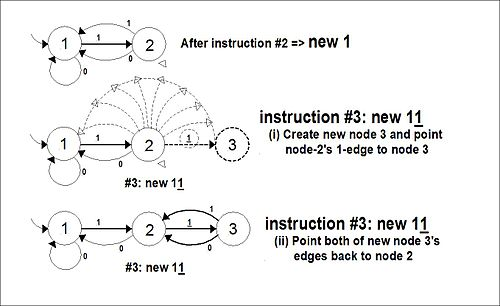
\includegraphics[width=300px]{pictures/pointer_machine.jpeg} \\
    \textit{Малополезная картинка}
\end{tabular}
\end{centering}


\tb{Full персистентный массив.} Давайте создадим двоичное дерево над массивом размера $n$ с высотой $O(\log n)$, реализовав его как pointer machine. Тогда теперь мы можем сделать изменение произвольного элемента в произвольной версии, получив $O(\log n)$ времени работы (и очевидную реализацию персистентного ДО в придачу).

\tb{Персистентное декартово дерево}. \\

Заметим, что наше декартово дерево можно было бы реализовать через pointer machine, что даст нам что-то очень похожее на то, что мы хотим от такой структуры данных. К сожалению, такая структура данных не будет $functional\ persistent$, потому что есть конструктивный способ очень сильно расширить дерево в высоту (достаточно просто мерджить одну и ту же вершину с последней версией дерева, получая бамбук).

Проблема у нас возникла в тот момент, когда мы воспользовалиь старой идеей приоритетов. Теперь будем вычислять что-то типа приоритетов динамически. А именно, будем считать, что приоритет дерева $L$ больше приоритета дерева $R$, если $rand() < \frac{S(L)}{S(L) + S(R)}$. Можно показать, что теперь высота ДД все еще $O(\log n)$.

\end{document}